\documentclass[]{elsarticle} %review=doublespace preprint=single 5p=2 column
%%% Begin My package additions %%%%%%%%%%%%%%%%%%%
\usepackage[hyphens]{url}

  \journal{Global Health Research and Policy - Thematic Series: Universal Health Coverage} % Sets Journal name


\usepackage{lineno} % add
\providecommand{\tightlist}{%
  \setlength{\itemsep}{0pt}\setlength{\parskip}{0pt}}

\bibliographystyle{elsarticle-harv}
\biboptions{sort&compress} % For natbib
\usepackage{graphicx}
\usepackage{booktabs} % book-quality tables
%%%%%%%%%%%%%%%% end my additions to header

\usepackage[T1]{fontenc}
\usepackage{lmodern}
\usepackage{amssymb,amsmath}
\usepackage{ifxetex,ifluatex}
\usepackage{fixltx2e} % provides \textsubscript
% use upquote if available, for straight quotes in verbatim environments
\IfFileExists{upquote.sty}{\usepackage{upquote}}{}
\ifnum 0\ifxetex 1\fi\ifluatex 1\fi=0 % if pdftex
  \usepackage[utf8]{inputenc}
\else % if luatex or xelatex
  \usepackage{fontspec}
  \ifxetex
    \usepackage{xltxtra,xunicode}
  \fi
  \defaultfontfeatures{Mapping=tex-text,Scale=MatchLowercase}
  \newcommand{\euro}{€}
\fi
% use microtype if available
\IfFileExists{microtype.sty}{\usepackage{microtype}}{}
\usepackage[left=3cm,right=3cm,top=3cm,bottom=3cm]{geometry}
\usepackage{longtable}
\usepackage{graphicx}
% We will generate all images so they have a width \maxwidth. This means
% that they will get their normal width if they fit onto the page, but
% are scaled down if they would overflow the margins.
\makeatletter
\def\maxwidth{\ifdim\Gin@nat@width>\linewidth\linewidth
\else\Gin@nat@width\fi}
\makeatother
\let\Oldincludegraphics\includegraphics
\renewcommand{\includegraphics}[1]{\Oldincludegraphics[width=\maxwidth]{#1}}
\ifxetex
  \usepackage[setpagesize=false, % page size defined by xetex
              unicode=false, % unicode breaks when used with xetex
              xetex]{hyperref}
\else
  \usepackage[unicode=true]{hyperref}
\fi
\hypersetup{breaklinks=true,
            bookmarks=true,
            pdfauthor={},
            pdftitle={Association between compulsory health insurance and life expectancy in 184 countries: A retrospective longitudinal study},
            colorlinks=true,
            urlcolor=blue,
            linkcolor=blue,
            pdfborder={0 0 0}}
\urlstyle{same}  % don't use monospace font for urls

\setcounter{secnumdepth}{5}
% Pandoc toggle for numbering sections (defaults to be off)
% Pandoc header
\usepackage{soulutf8}
\usepackage{color}
\usepackage{float}
\usepackage{booktabs}
\usepackage{lscape}
\usepackage{setspace}
\usepackage{dcolumn}



\begin{document}
\begin{frontmatter}

  \title{Association between compulsory health insurance and life expectancy in 184 countries: A retrospective longitudinal study}
    \author[SLU]{Miao Cai}
   \ead{miao.cai@slu.edu} 
  
    \author[SLU]{Asabe Garba}
   \ead{asabe.garba@slu.edu} 
  
    \author[SCU]{Xiaojun Lin\corref{c1}}
   \ead{xjlin@hust.edu.cn} 
   \cortext[c1]{Corresponding Author}
    \author[WHU]{Xin Li}
   \ead{xl60@iu.edu} 
  
    \author[SLU]{Ziqi Peng}
   \ead{ziqi.peng@slu.edu} 
  
    \author[SLU]{Thembekile Shato}
   \ead{thembekile.shato@slu.edu} 
  
    \author[SLU]{Ucheoma Nwaozuru}
   \ead{ucheoma.nwaozuru@slu.edu} 
  
      \address[SLU]{College for Public Health and Social Justice, Saint Louis University, Saint Louis, MO, 63108}
    \address[SCU]{West China School of Public Health, Sichuan University, Chengdu, Sichuan, China, 610041}
    \address[WHU]{School of Information Management, Wuhan University, Wuhan, Hubei, China, 430072}
  
  \begin{abstract}
  \textbf{Background: } Wide discrepancies in life expectancy still exist across the world due to variations in income levels and educational attainment. The objective of this study is to investigate the association between compulsory health insurance and life expectancy and whether there are heterogeneous impacts on life expectancy among different income groups.\\
  \textbf{Methods: } Country-level data for 184 countries from the Global Health Expenditure Database from 2000 to 2016 were used in this study. Ordinary least square models were applied to esitmate the association between compulsory health insurance and life expectancy, adjusting for country level characteristics, health expenditure and other health financing arrangements.\\
  \textbf{Results: } A total of 2,975 complete country-year observations from 184 countries were included in this study. One percent increase in compulsory health insurance as percent of current health expenditure (CHE) was associated with 0.035 years (95\% CI: {[}0.025, 0.045{]}) increase in life expectancy overall. In the subgroup analysis of country income group, we found that the percent of compulsory health insurance is positively associated with life expectancy among low (\(\beta = 0.224\), 95\% CI: {[}0.055, 0.392{]}), low-mid (\(\beta = 0.243\), 95\% CI: {[}0.195, 0.291{]}), and up-mid income (\(\beta = 0.061\), 95\% CI: {[}0.045, 0.078{]}) countries. However, this association turned out to be negative among high income countries (\(\beta = -0.011\), 95\% CI: {[}-0.018, 0.005{]}).\\
  \textbf{Conclusion: } Compulsory health insurance is associated with life expectancy in 184 countries. Increasing the compulsory health insurance as percentage of CHE may improve life expectancy among low and middle income countries.
  \end{abstract}
  
 \end{frontmatter}

\newcommand{\blandscape}{\begin{landscape}}
\newcommand{\elandscape}{\end{landscape}}
\doublespacing

\hypertarget{introduction}{%
\section{Introduction}\label{introduction}}

Life expectancy is defined as the average number of years that a person will live from birth based on measures such as birth year, gender, and current age. This calculation assumes that mortality rates will remain the same as time progresses. The greatest factors that impact life expectancy overall include income, quality of public health, medical care, and diet. {[}\protect\hyperlink{ref-Statista}{1}{]}.
Due to increasing rates of economic growth and access to health care coverage, life expectancy at birth and healthy life expectancy have significantly risen worldwide {[}\protect\hyperlink{ref-bor2013increases}{2}, \protect\hyperlink{ref-mathers2015causes}{3}{]}.
However, life expectancy disparities still exist across the world due to variations in income level and educational attainment {[}\protect\hyperlink{ref-world2018global}{4}{]}.
According to the World Health Organization (WHO), the average life expectancy globally in 2016 was 72 years of age. Global life expectancy ranged from 61.2 years in the African Region to 77.5 years in the European Region, a ratio of 1.3 between the regions {[}\protect\hyperlink{ref-WHOobserve}{5}{]}.

Employment, education, diet, quality of life, environmental conditions, government health expenditure, and income have been reported as the main risk factors that have significant effects on life expectancy in both developed and developing countries {[}\protect\hyperlink{ref-assari2018life}{6}--\protect\hyperlink{ref-wilkinson2018impact}{12}{]}.
Among these risk factors, poverty (income level) is the primary cause of ill-health and decreased life expectancy due to its negative effect on environmental sustainability and insufficient access to health care services {[}\protect\hyperlink{ref-world2001dying}{13}--\protect\hyperlink{ref-rehm2018drinking}{15}{]}.
Globally, approximately 1.2 billion people live in extreme poverty, and 2.7 billion live in moderate poverty {[}\protect\hyperlink{ref-olinto2013state}{16}{]}.
In order to decrease share of out-of-pocket spending and ensure health care access to economically disadvantaged populations, health insurance coverage and prepayment schemes have been widely established in health care systems around the world {[}\protect\hyperlink{ref-wagstaff2018progress}{17}{]}.
In developing countries, compulsory health insurance has been successfully implemented u as a tool for concentrating resources in the health sector and providing needed medical service to low-income households {[}\protect\hyperlink{ref-abel1992health}{18}--\protect\hyperlink{ref-meng2015consolidating}{22}{]}.

There is growing attention on compulsory health insurance because it has been proven as an effective way to achieve Universal Health Coverage {[}\protect\hyperlink{ref-wagstaff2018progress}{17}{]}.
Compulsory health insurance, also known as the Bismarck Sickness Insurance, was first introduced in Germany in 1883.
It guaranteed that all workers and their families had access to health services {[}\protect\hyperlink{ref-walker1969compulsory}{23}{]}.
Australia (1888), Hungary (1891), England (1911), and Japan (1922) respectively all later adopted national compulsory health insurance systems as well {[}\protect\hyperlink{ref-walker1969compulsory}{23}{]}.
Most countries in the world either use national compulsory insurance plans or a similar type of health care system {[}\protect\hyperlink{ref-healthglance2017}{24}{]}.
Health care spending accounts for the use of health care services and public health services.
As a result, there is a clear trend in the relationship between compulsory health insurance and the life expectancy in a country.
As a country's health expenditure increases, the life expectancy also increases.
However, to the best of our knowledge, the exploration of the long-term impact of compulsory health insurance on life expectancy is limited.
This includes looking at the association between compulsory health insurance and life expectancy in different countries.
The strength and changes related to this association have not been systematically investigated and compared.

This study addressed the main gaps that exist in previous literature on the association between compulsory health insurance and life expectancy among different countries over time. Using country-level longitudinal data from years 2000 to 2016, the purpose of this study was to examine the association between compulsory health insurance and life expectancy and to also explore the different patterns of this association in low, low-mid, up-mid, and high-income countries respectively.

\hypertarget{methods}{%
\section{Methods}\label{methods}}

\hypertarget{data-source}{%
\subsection{Data source}\label{data-source}}

The country level data that was used for this study was extracted from the Global Health Expenditure Database {[}\protect\hyperlink{ref-WHOdata}{25}{]}.
This database is sponsored by the World Health Organization (WHO) and provides health expenditure data on 190 countries from years 2000 to 2016.
The current health expenditure (CHE) can be decomposed into several variables: domestic government health expenditure, private health expenditure, and percentage of out-of-pocket (OOP) payment;
financing arrangements can be decomposed into the variables compulsory financing arrangements, government financing arrangements, compulsory health insurance, household OOP payment as a percent of CHE;
CHE and government health expenditure as a percent of gross domestic product (GDP).

In addition to looking at specific decomposed variables for health expenditure and financing arrangements, we looked at the countries in the World Bank Open Data and extracted life expectancy, GDP, and population data from years 2000 to 2016 {[}\protect\hyperlink{ref-worldbank}{26}{]}.
Both databases are publicly available, with downloadable comma-separated values or Microsoft Excel files provided on the WHO website.
The two databases were then merged according to two common keys, country name and year, in order to perform our analyses.

\hypertarget{variable-selection}{%
\subsection{Variable selection}\label{variable-selection}}

The outcome variable, life expectancy at birth in a specific year, was assessed for each country.
It reflected the overall mortality rate of all age groups in a given year by country.
Life expectancy is one of the most widely used measures of mortality and burden of disease in previous literature {[}\protect\hyperlink{ref-mathers2015causes}{3}, \protect\hyperlink{ref-lee2012effect}{27}--\protect\hyperlink{ref-bennett2015future}{29}{]}.

We included three key sets of explanatory variables to predict life expectancy in the 184 countries over time.
Country level general characteristics included population (in millions), year (2000 to 2015), and GDP (in billions).
The GDP data were reported in constant 2010 prices, which were adjusted for the effects of price inflation {[}\protect\hyperlink{ref-worldbankconstant}{30}{]}.
Current health expenditure (CHE) and government health expenditure (GGHE-D) as percent of GDP were used to account for investment in healthcare for a given country.
Compulsory financing arrangements and compulsory health insurance as percent of the CHE were also included to account for any differences in the source of financing arrangements.
Private health expenditure and OOP payment as percent of the CHE were two sources of healthcare expenditure.
These percents fell in the range of 0 to 100. We excluded variables that could cause multicollinearity in our statistical models, which was determined by the variance inflation factor.

The income group of a country was classified into four groups based on the World Bank's classification criterion for that fiscal year: low, low-mid, up-mid, and high {[}\protect\hyperlink{ref-worldbankincome}{31}{]}. This income classification for each country is based on the national income per person in a year and can vary by year {[}\protect\hyperlink{ref-worldbankincome}{31}{]}.
The year variable was not converted into dummy variables for two reasons: firstly, since there were 16 years of data, creating 15 dummy variables may exhaust the degrees of freedom in our statistical models, especially in stratified analyses; secondly, the life expectancy in different countries was generally linearly correlated with year, as shown in Figure \ref{fig:fig1}.

\hypertarget{statistical-analyses}{%
\subsection{Statistical Analyses}\label{statistical-analyses}}

Observations with missing data in either the dependent variable or any of the explanatory variables were excluded, resulting in a total of 2,975 complete observations (91\% of the original data) from 184 countries.
Since only 166 of the 184 countries (90.2\%) had complete data in the seventeen-year period (2000 to 2016), our empirical analysis relied on unbalanced country-level panel data.
Among the 184 sample countries, there were 49 in the African Region, 35 in the American Region, 19 in the South-East Asia Region, 51 in the European Region, 10 in the Eastern Mediterranean Region, and 23 in the Western Pacific Region {[}\protect\hyperlink{ref-WHOregion}{32}{]}.

We estimated the association between compulsory health insurance and life expectancy among the 184 countries using an ordinary least square model that accounted for all the covariates and time trend fixed-effects.
Since high- and low-income countries can be characterized by different patterns of life expectancy and health financing schemes, we conducted stratified analyses among the four income category countries to allow for potentially different patterns of association between compulsory health insurance and life expectancy among the 184 countries.
Our main hypothesis was that compulsory health insurance was positively associated with life expectancy.

We reported point and interval estimates (95\% confidence intervals, 95\% CI), as well as the significance of all independent variables.
A p-value less than 0.05 was viewed as statistically significant.
All data cleaning, visualization, statistical modelling, and reporting were performed with the use of R software, version 3.5.3 (R Foundation for Statistical Computing) {[}\protect\hyperlink{ref-R353}{33}{]}.
In an effort to promote reproducible research, we created a public GitHub repository to store all the data and R code we used to write this paper.
Interested readers can find them at \url{https://github.com/caimiao0714/GHRP-UHC}.

\hypertarget{results}{%
\section{Results}\label{results}}

\hypertarget{characteristics-of-the-countries-by-income-group}{%
\subsection{Characteristics of the countries by income group}\label{characteristics-of-the-countries-by-income-group}}

\begin{table}[H]

\caption{\label{tab:descriptive}Characteristics of the 184 countries by income group, 2000 - 2016}
\centering
\resizebox{\linewidth}{!}{
\begin{tabular}{llllll}
\toprule
  & Overall & Low & Low-Mid & Up-Mid & High\\
\midrule
No of observations & 2975 & 459 & 830 & 826 & 860\\
Life expectancy & 69.27 (9.09) & 56.65 (5.59) & 65.45 (7.26) & 71.22 (5.71) & 77.82 (3.35)\\
Compulsory health insurance as percent of CHE & 13.86 (22.08) & 1.35 (2.53) & 6.58 (9.78) & 18.06 (22.52) & 23.53 (29.31)\\
Current health expenditure as percent of GDP & 6.12 (2.53) & 6.15 (2.46) & 5.36 (2.35) & 5.74 (2.15) & 7.21 (2.70)\\
Government Health Expenditure as percent of GDP & 3.20 (2.17) & 1.40 (0.74) & 2.26 (1.66) & 3.18 (1.64) & 5.09 (2.15)\\
\addlinespace
Private health expenditure as percent CHE & 41.38 (19.62) & 49.91 (18.30) & 47.83 (22.12) & 42.65 (17.53) & 29.39 (12.74)\\
Out-of-pocket payment as percent of CHE & 35.08 (19.78) & 44.73 (18.82) & 43.37 (21.81) & 35.00 (17.77) & 22.00 (10.76)\\
Compulsory financing arrangements as percent of CHE & 53.02 (21.69) & 36.18 (14.99) & 46.49 (21.04) & 55.40 (17.48) & 66.01 (20.50)\\
Population (millions) & 37.92 (138.36) & 17.71 (19.03) & 54.24 (172.60) & 48.99 (188.88) & 22.34 (47.24)\\
GDP & 35.47 (134.11) & 0.90 (0.86) & 8.54 (24.51) & 28.61 (89.20) & 86.51 (223.73)\\
\bottomrule
\multicolumn{6}{l}{Means and standard deviations (in parentheses) are reported. GDP: Gross Domestic Product; CHE: Current Health Expenditure}\\
\end{tabular}}
\end{table}

\begin{figure}
\centering
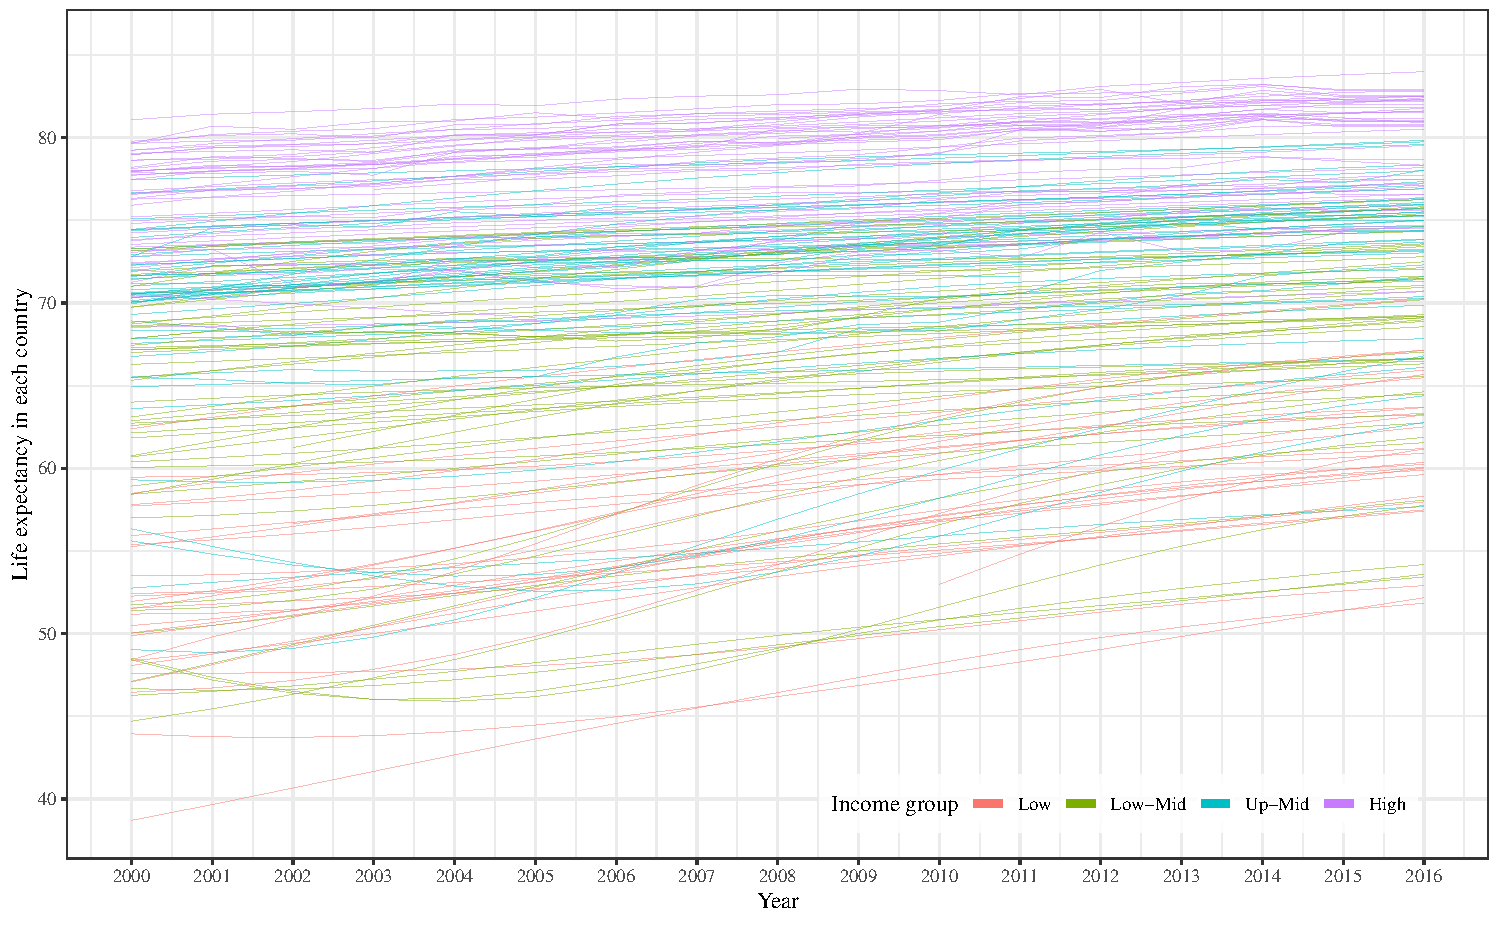
\includegraphics{Figures/fig1.pdf}
\caption{\label{fig:fig1}Life expectancy in 184 countries stratified by country income group, 2000 - 2016}
\end{figure}

Table \ref{tab:descriptive} presents averages and standard deviations (in parentheses) for the different characteristics of the 184 countries stratified by income group.
High-income countries had the highest average life expectancy (77.82 years), followed by up-mid (71.22 years), low-mid (65.45 years), and low-income countries (56.65 years).
Figure \ref{fig:fig1} shows the trends of life expectancy in the 184 countries over the seventeen-year period, with each line representing a country and each color an income category.
The life expectancy in the studied countries were generally linear with a clear increase from 2000 to 2016.
Consistent with Table \ref{tab:descriptive} results, the most significant pattern in the plot was that life expectancy was strongly related to income group: the high-income countries had the highest life expectancy, which increased from about 77 in 2000 to around 80 years old in 2016;
the low-income countries generally had the lowest life expectancy, which increased from around 50 to about 58 years old.
The gap of life expectancy between high- and low-income countries narrowed from 2000 to 2016.
It was also to be noted that the variance of life expectancy in low and low-mid income countries were much higher than that in up-mid and high-income countries.

Regarding healthcare expenditure, it appeared that lower income countries had less government health expenditure as percent of GDP, more private health expenditure, and OOP payments as percent of GDP, compared to higher income countries. In terms of financing arrangement, higher income countries had a higher percent of compulsory financing arrangements and compulsory health insurance as percent of current health expenditure. Compared to low-mid and up-mid income countries, high- and low-income countries had smaller populations but more current health expenditure as percent of GDP.

\hypertarget{potential-life-expectancy-gain-by-compulsory-health-insurance}{%
\subsection{Potential life expectancy gain by compulsory health insurance}\label{potential-life-expectancy-gain-by-compulsory-health-insurance}}

\begin{table}[H] \centering 
  \caption{OLS model predicting life expectancy in 184 countries, 2000 - 2016} 
  \label{poolOLS} 
\begin{tabular}{@{\extracolsep{5pt}}lc} 
\\[-1.8ex]\hline \\[-1.8ex] 
\\[-1.8ex] & Life expectancy \\ 
\hline \\[-1.8ex] 
 Compulsory health insurance as percent of CHE & 0.035$^{***}$ \\ 
  & (0.025, 0.045) \\ 
  Current health expenditure as percent of GDP & 0.162$^{*}$ \\ 
  & (0.026, 0.298) \\ 
  Government health expenditure as percent of GDP & 0.482$^{***}$ \\ 
  & (0.263, 0.702) \\ 
  Private health expenditure as percent CHE & $-$0.154$^{***}$ \\ 
  & ($-$0.186, $-$0.122) \\ 
  Out-of-pocket payment as percent of CHE & 0.174$^{***}$ \\ 
  & (0.146, 0.201) \\ 
  Compulsory financing arrangements as percent of CHE & 0.0003 \\ 
  & ($-$0.016, 0.017) \\ 
  Population (millions) & 0.002$^{**}$ \\ 
  & (0.001, 0.004) \\ 
  GDP & 0.001 \\ 
  & ($-$0.0003, 0.003) \\ 
  Year & 0.301$^{***}$ \\ 
  & (0.263, 0.339) \\ 
  Low income country & $-$19.084$^{***}$ \\ 
  & ($-$19.889, $-$18.280) \\ 
  Low to middle income country & $-$10.936$^{***}$ \\ 
  & ($-$11.539, $-$10.334) \\ 
  Up to middle income country & $-$5.414$^{***}$ \\ 
  & ($-$5.945, $-$4.882) \\ 
  Constant & $-$529.862$^{***}$ \\ 
  & ($-$605.762, $-$453.961) \\ 
 \textit{N} & 2,975 \\ 
R$^{2}$ & 0.695 \\ 
Adjusted R$^{2}$ & 0.694 \\ 
\hline \\[-1.8ex] 
\multicolumn{2}{l}{$^{*}$p $<$ .05; $^{**}$p $<$ .01; $^{***}$p $<$ .001} \\ 
\multicolumn{2}{l}{GDP: Gross Domestic Product} \\ 
\multicolumn{2}{l}{CHE: Current Health Expenditure} \\ 
\end{tabular} 
\end{table}

Table \ref{poolOLS} presents the overall relationship between compulsory health insurance and life expectancy. Controlling for other covariates, there was a one percent increase in compulsory health insurance as percent of CHE that was associated with a 0.035 year (95\% CI: {[}0.025, 0.045{]}) increase in overall life expectancy. The CHE and GGHE-D as percent of GDP were positively associated with life expectancy. The countries with higher OOP as percent of CHE and lower private health expenditure as percent CHE had higher life expectancies. Compulsory financing arrangements as percent of CHE did not appear to be a significant predictor. In addition, a larger population size was associated with a higher life expectancy, although the
coefficient was small. Compared to high-income countries, the life expectancy in low-income as well as the low to middle-income and up to middle-income countries was significantly lower. It was worth noting that the effect size for low-income countries (\(\beta = -19.084\), 95\% CI: {[}-19.889, -18.280{]}) was much larger than the low to middle-income (\(\beta = -10.936\), 95\% CI: {[}-11.539, -10.334{]}) and up to middle-income countries (\(\beta = -5.414\), 95\% CI: {[}-5.945, -4.882{]}), after controlling for potential covariates.

\hypertarget{potential-life-expectancy-gain-by-compulsory-health-insurance-in-different-income-groups}{%
\subsection{Potential life expectancy gain by compulsory health insurance in different income groups}\label{potential-life-expectancy-gain-by-compulsory-health-insurance-in-different-income-groups}}

Table \ref{stratifiedOLS} ppresents the relationship between compulsory health insurance as percent of CHE and life expectancy in the different countries by income group. The percent of compulsory health insurance was positively associated with life expectancy among low (\(\beta = 0.224\), 95\% CI: {[}0.055, 0.392{]}), low-mid (\(\beta = 0.243\), 95\% CI: {[}0.195, 0.291{]}), and up-mid income (\(\beta = 0.061\), 95\% CI: {[}0.045, 0.078{]}) countries. However, this association was found negative among high-income countries (\(\beta = -0.011\), 95\% CI: {[}-0.018, 0.005{]}), , although the effect size was very small.

The effects of predictors on life expectancy varied across income groups. CHE as percent of GDP was found to be positively correlated with life expectancy in the up-mid income countries. However, this correlation was negative in high-income countries. Similarly, the effect of GGHE-D as percent of GDP on life expectancy changed from negative in up-mid countries to positive in high-income countries. Private Health Expenditure as percent CHE was positively associated with life expectancy among low- and high-income countries but was negatively associated with life expectancy among low-mid and up-mid income countries. For low- and high-income countries, OOP as percent of CHE had negative effects on life expectancy. However, the effect of OOP as percent of CHE on life expectancy was positive among low-mid and up-mid income countries.

\begin{landscape}

\begin{table}[!] \centering 
  \caption{OLS model predicting life expectancy, 2000 - 2016, stratified by country income categories, } 
  \label{stratifiedOLS} 
\begin{tabular}{@{\extracolsep{5pt}}lD{.}{.}{-3} D{.}{.}{-3} D{.}{.}{-3} D{.}{.}{-3} } 
\\[-1.8ex]\hline \\[-1.8ex] 
\\[-1.8ex] & \multicolumn{4}{c}{Life expectancy} \\ 
 & \multicolumn{1}{c}{Low} & \multicolumn{1}{c}{Low-mid} & \multicolumn{1}{c}{Up-mid} & \multicolumn{1}{c}{High} \\ 
\\[-1.8ex] & \multicolumn{1}{c}{Model 1} & \multicolumn{1}{c}{Model 2} & \multicolumn{1}{c}{Model 3} & \multicolumn{1}{c}{Model 4}\\ 
\hline \\[-1.8ex] 
 Compulsory health insurance as percent of CHE & 0.224^{**} & 0.243^{***} & 0.061^{***} & -0.011^{***} \\ 
  & \multicolumn{1}{c}{(0.055$, $0.392)} & \multicolumn{1}{c}{(0.195$, $0.291)} & \multicolumn{1}{c}{(0.045$, $0.078)} & \multicolumn{1}{c}{(-0.018$, $-0.005)} \\ 
  Current Health Expenditure as percent of GDP & -0.155 & 0.157 & 1.022^{***} & -0.719^{***} \\ 
  & \multicolumn{1}{c}{(-0.377$, $0.067)} & \multicolumn{1}{c}{(-0.122$, $0.436)} & \multicolumn{1}{c}{(0.595$, $1.448)} & \multicolumn{1}{c}{(-1.039$, $-0.399)} \\ 
  Government Health Expenditure as percent of GDP & -0.394 & 0.099 & -0.890^{*} & 1.975^{***} \\ 
  & \multicolumn{1}{c}{(-1.189$, $0.402)} & \multicolumn{1}{c}{(-0.391$, $0.590)} & \multicolumn{1}{c}{(-1.597$, $-0.183)} & \multicolumn{1}{c}{(1.554$, $2.397)} \\ 
  Private Health Expenditure as percent CHE & 0.174^{***} & -0.373^{***} & -0.137^{***} & 0.116^{***} \\ 
  & \multicolumn{1}{c}{(0.087$, $0.262)} & \multicolumn{1}{c}{(-0.469$, $-0.277)} & \multicolumn{1}{c}{(-0.215$, $-0.059)} & \multicolumn{1}{c}{(0.072$, $0.159)} \\ 
  Out-of-pocket payment as percent of CHE & -0.172^{***} & 0.435^{***} & 0.239^{***} & -0.043^{*} \\ 
  & \multicolumn{1}{c}{(-0.254$, $-0.090)} & \multicolumn{1}{c}{(0.349$, $0.520)} & \multicolumn{1}{c}{(0.201$, $0.277)} & \multicolumn{1}{c}{(-0.076$, $-0.010)} \\ 
  Compulsory Financing Arrangements as percent of CHE & -0.024 & 0.054 & 0.148^{***} & 0.002 \\ 
  & \multicolumn{1}{c}{(-0.075$, $0.026)} & \multicolumn{1}{c}{(-0.008$, $0.116)} & \multicolumn{1}{c}{(0.087$, $0.210)} & \multicolumn{1}{c}{(-0.009$, $0.012)} \\ 
  Population (millions) & -0.056^{*} & -0.005 & 0.003 & 0.012 \\ 
  & \multicolumn{1}{c}{(-0.100$, $-0.012)} & \multicolumn{1}{c}{(-0.012$, $0.002)} & \multicolumn{1}{c}{(-0.001$, $0.007)} & \multicolumn{1}{c}{(-0.009$, $0.032)} \\ 
  GDP & 2.435^{***} & 0.060^{*} & 0.001 & -0.003 \\ 
  & \multicolumn{1}{c}{(1.427$, $3.444)} & \multicolumn{1}{c}{(0.011$, $0.109)} & \multicolumn{1}{c}{(-0.007$, $0.009)} & \multicolumn{1}{c}{(-0.007$, $0.002)} \\ 
  Year & 0.506^{***} & 0.289^{***} & 0.225^{***} & 0.158^{***} \\ 
  & \multicolumn{1}{c}{(0.409$, $0.602)} & \multicolumn{1}{c}{(0.200$, $0.378)} & \multicolumn{1}{c}{(0.160$, $0.290)} & \multicolumn{1}{c}{(0.122$, $0.195)} \\ 
  Constant & -958.790^{***} & -521.271^{***} & -395.563^{***} & -247.217^{***} \\ 
  & \multicolumn{1}{c}{(-1,152.821$, $-764.759)} & \multicolumn{1}{c}{(-699.343$, $-343.198)} & \multicolumn{1}{c}{(-525.258$, $-265.868)} & \multicolumn{1}{c}{(-319.848$, $-174.585)} \\ 
 \textit{N} & \multicolumn{1}{c}{459} & \multicolumn{1}{c}{830} & \multicolumn{1}{c}{826} & \multicolumn{1}{c}{860} \\ 
R$^{2}$ & \multicolumn{1}{c}{0.391} & \multicolumn{1}{c}{0.304} & \multicolumn{1}{c}{0.385} & \multicolumn{1}{c}{0.465} \\ 
Adjusted R$^{2}$ & \multicolumn{1}{c}{0.379} & \multicolumn{1}{c}{0.296} & \multicolumn{1}{c}{0.378} & \multicolumn{1}{c}{0.460} \\ 
\hline \\[-1.8ex] 
\multicolumn{5}{l}{$^{*}$p $<$ .05; $^{**}$p $<$ .01; $^{***}$p $<$ .001} \\ 
\multicolumn{5}{l}{GDP: Gross Domestic Product} \\ 
\multicolumn{5}{l}{CHE: Current Health Expenditure} \\ 
\end{tabular} 
\end{table} 
\end{landscape}

\hypertarget{discussion}{%
\section{Discussion}\label{discussion}}

In this study, we explored the association between compulsory health insurance and life expectancy in 184 countries over a 17-year period.
Our regression models revealed that compulsory health insurance was significantly associated with life expectancy, after adjusting for country level characteristics, health expenditure, and other health financing arrangements.
Furthermore, compulsory health insurance had positive effects on life expectancy among low, low-mid and up-mid countries, while negative effects among high income countries.

It is interesting that the association between compulsory health insurance and life expectancy was different among high income and not high income countries. A positive association between compulsory health insurance and life expectancy was found among low, low-mid, upper-mid countries, which was consistent with previous literature. For example, several studies conducted in Vietnam, a low-mid income country as classified by the World Bank {[}\protect\hyperlink{ref-worldbankincome}{31}{]}, have reported the positive association between health insurance coverage and health outcomes {[}\protect\hyperlink{ref-jowett2003impact}{20}, \protect\hyperlink{ref-jowett2004health}{34}--\protect\hyperlink{ref-Nguyen2012}{36}{]}. Compulsory health insurance is generally encouraged in low and middle income countries to achieve universal coverage, purchase services, and pool risk {[}\protect\hyperlink{ref-barnighausen2002one}{37}, \protect\hyperlink{ref-lagomarsino2012moving}{38}{]}.

There are several possible explanations for the positive assocation between compulsory health insurance and life expectancy. First, increasing the compulsory health insurance as percent of CHE may increase the enrollees' accessibility to health service. Using the introduction of compulsory health insurance in the German Empire in 1884 as a natural experiment, Stefan and colleagues investigated the association between Bismarck's health insurance and the mortality. They aruged that the Bismarck's health insurance reduced mortality significantly, which could be largely explained by an increase in access to health service {[}\protect\hyperlink{ref-bauernschuster2017bismarck}{39}{]}. Curtis developed a cohort study of patients with cystic fibrosis, and they found that the absence of health insurance is associated with decreased life expectancy {[}\protect\hyperlink{ref-Curtis1997}{40}{]}.

Second, the improving health utilization brought by health insurance may partially explain the gains in life expectancy. Freeman argued that health insurance had significant effects on increasing health utilization, especially on the use of physician services and preventive services, and improving health outcomes, such as self-reported health status and mortality {[}\protect\hyperlink{ref-Freeman2008}{41}{]}. In China, a typical up-mind income country, Pan et al.~found that the beneficiaries of the Urban Resident Basic Medical Insurance had better health than the uninsured {[}\protect\hyperlink{ref-Pan2016}{42}{]}. Using data from Vietnam, Nguyen reported that participating the voluntary health insurance was associated with the annual outpatient and inpatient visits {[}\protect\hyperlink{ref-Nguyen2012}{36}{]}.

Most high income countries have a national health insurance system, such as Canada, Germany, the United Kingdom, Japan, with the only exception of the United States {[}\protect\hyperlink{ref-Emery2010}{43}{]}. Compared to low and middle income countries, they have various alternative approaches to fund health expenditure for their citizens, such as employer provided health insurance {[}\protect\hyperlink{ref-lagomarsino2012moving}{38}{]}. In contrast to results found among low and middle income countries, we found a negative association between compulsory health insurance and life expectancy among high income countries. Two mechanism may potentially explain this different association. First, economic theory explains that compulsory health insurance schemes expands insurance coverage, but creates additional burden for household and reduces consumer's ability to purchase other items {[}\protect\hyperlink{ref-koch2010health}{44}{]}. This reallocation of household expenditure may result in greater effects compared to compulsory health insurance benefits. Second, although compulsory health insurance schemes has potential benefits of purchase service and pooling risk, the relative efficiency of them compared to private insurance schemes are to be doubted {[}\protect\hyperlink{ref-savedoff2012political}{45}{]}. An example is the National Health Service in the United Kingdom, which experienced several round of reforms that targeted improving market competition, quality and efficiency of health care providers {[}\protect\hyperlink{ref-bevan2011does}{46}, \protect\hyperlink{ref-gaynor2013death}{47}{]}. Although the negative association among high income countries was statistically significant, the effect size was small (-0.011) compared to the other three estimates (0.224 for low income countries, 0.243 for low-mid income countries, and 0.061 for up-mid income countries). This likely results from the small variance of life expectancy in high income countries, as shown in Figure \ref{fig:fig1}.

This study contributes to the body of evidence on insurance and life expectancy in the following aspects. First, although the association between health insurance and life expectancy has been investigated in previous works{[}\protect\hyperlink{ref-bauernschuster2017bismarck}{39}, \protect\hyperlink{ref-Curtis1997}{40}{]}, few studies shed lights on the gains in life expectancy from increasing the percentage of compulsory health insurance in current health expenditure. Our study fills this research gap by using country-level longitudinal data. Second, empirical studies on insurance and life expectancy were confined to a specific country or region, such as the United States and Germany {[}\protect\hyperlink{ref-bauernschuster2017bismarck}{39}, \protect\hyperlink{ref-Curtis1997}{40}{]}. Given that the health insurance systems vary substaintially across countries, more research is needed to examine the association in multiple countries. To the best of our knowledge, this is the first study to assess the impact of compulsory health insuance on life expectancy among a large number of countries.

Our study had several limitations. First, the relationships between compulsory health insurance and life expectancy should not be interpreted as causal effects dut to the design of observational study. To conduct causal inference in future studies, researcher can use quasi-experimental design and modern econometric models, such as instrumental variables and regression discontinuity design, to explore the causal effects of compulsory health insurance scheme. Second, our results might be confounded by unmeasured factors, including the sanitation facilities, water and air quality, life style, medical resources and literacy level. Due to data unavailability, we were unable to include these individual or regional level data in our analyses. Therefore, further research based on more comprehensive databases may provide more robust results. Third, although the association between complusory health insurance and life expectancy was unveiled in this study, the underlying mechanisms remain unclear.

\hypertarget{conclusion}{%
\section{Conclusion}\label{conclusion}}

This study demostrates that in the period 2000-2016, compulsory health insurance is associated with life expectancy in 184 countries. Increasing the compulsory health insurance as percentage of CHE may improve life expectancy and should be considered as a way of improving population health for low and low-mid income countries.

\hypertarget{acknowledgements}{%
\section*{Acknowledgements}\label{acknowledgements}}
\addcontentsline{toc}{section}{Acknowledgements}

We thank the WHO and the World Bank for making the data used in this study publicly available for researchers.

\hypertarget{funding}{%
\section*{Funding}\label{funding}}
\addcontentsline{toc}{section}{Funding}

None.

\hypertarget{availability-of-data-and-materials}{%
\section*{Availability of data and materials}\label{availability-of-data-and-materials}}
\addcontentsline{toc}{section}{Availability of data and materials}

All data and associated R code are public available at the GitHub repository \texttt{caimiao0714/GHRP-UHC}, which can be accessed at \url{https://github.com/caimiao0714/GHRP-UHC}.

\hypertarget{references}{%
\section*{References}\label{references}}
\addcontentsline{toc}{section}{References}

\hypertarget{refs}{}
\leavevmode\hypertarget{ref-Statista}{}%
1. Statista. Life expectancy by continent 2018. 2018. \url{https://www.statista.com/statistics/270861/life-expectancy-by-continent/}. Accessed 20 Mar 2019.

\leavevmode\hypertarget{ref-bor2013increases}{}%
2. Bor J, Herbst AJ, Newell M-L, Bärnighausen T. Increases in adult life expectancy in rural south africa: Valuing the scale-up of hiv treatment. Science. 2013;339:961--5.

\leavevmode\hypertarget{ref-mathers2015causes}{}%
3. Mathers CD, Stevens GA, Boerma T, White RA, Tobias MI. Causes of international increases in older age life expectancy. The Lancet. 2015;385:540--8.

\leavevmode\hypertarget{ref-world2018global}{}%
4. World Health Organization. Management of Substance Abuse Unit. Global status report on alcohol and health, 2018. World Health Organization; 2018.

\leavevmode\hypertarget{ref-WHOobserve}{}%
5. The World Health Organization. Global Health Observatory (GHO) data: Life expectancy. 2016. \url{https://www.who.int/gho/mortality_burden_disease/life_tables/situation_trends/en/}. Accessed 20 Mar 2019.

\leavevmode\hypertarget{ref-assari2018life}{}%
6. Assari S. Life expectancy gain due to employment status depends on race, gender, education, and their intersections. Journal of racial and ethnic health disparities. 2018;5:375--86.

\leavevmode\hypertarget{ref-baker2011education}{}%
7. Baker DP, Leon J, Smith Greenaway EG, Collins J, Movit M. The education effect on population health: A reassessment. Population and development review. 2011;37:307--32.

\leavevmode\hypertarget{ref-cotlear2015overcoming}{}%
8. Cotlear D, Gómez-Dantés O, Knaul F, Atun R, Barreto IC, Cetrángolo O, et al. Overcoming social segregation in health care in latin america. The Lancet. 2015;385:1248--59.

\leavevmode\hypertarget{ref-schwartz2018estimating}{}%
9. Schwartz JD, Wang Y, Kloog I, Yitshak-Sade M, Dominici F, Zanobetti A. Estimating the effects of pm 2.5 on life expectancy using causal modeling methods. Environmental health perspectives. 2018;126:127002.

\leavevmode\hypertarget{ref-jakovljevic2016life}{}%
10. Jakovljevic MB, Vukovic M, Fontanesi J. Life expectancy and health expenditure evolution in eastern europe---did and dea analysis. Expert review of pharmacoeconomics \& outcomes research. 2016;16:537--46.

\leavevmode\hypertarget{ref-ranabhat2018influence}{}%
11. Ranabhat CL, Atkinson J, Park M-B, Kim C-B, Jakovljevic M. The influence of universal health coverage on life expectancy at birth (leab) and healthy life expectancy (hale): A multi-country cross-sectional study. Frontiers in pharmacology. 2018;9.

\leavevmode\hypertarget{ref-wilkinson2018impact}{}%
12. Wilkinson RG. The impact of income inequality on life expectancy. In: Locating health. Routledge; 2018. pp. 7--28.

\leavevmode\hypertarget{ref-world2001dying}{}%
13. Organization WH, others. Dying for change: Poor people's experience of health and ill-health. 2001.

\leavevmode\hypertarget{ref-ezeh2017history}{}%
14. Ezeh A, Oyebode O, Satterthwaite D, Chen Y-F, Ndugwa R, Sartori J, et al. The history, geography, and sociology of slums and the health problems of people who live in slums. The lancet. 2017;389:547--58.

\leavevmode\hypertarget{ref-rehm2018drinking}{}%
15. Rehm J, Probst C. What about drinking is associated with shorter life in poorer people? PLoS medicine. 2018;15:e1002477.

\leavevmode\hypertarget{ref-olinto2013state}{}%
16. Olinto P, Beegle K, Sobrado C, Uematsu H, others. The state of the poor: Where are the poor, where is extreme poverty harder to end, and what is the current profile of the world's poor. Economic Premise. 2013;125:1--8.

\leavevmode\hypertarget{ref-wagstaff2018progress}{}%
17. Wagstaff A, Flores G, Smitz M-F, Hsu J, Chepynoga K, Eozenou P. Progress on impoverishing health spending in 122 countries: A retrospective observational study. The Lancet Global Health. 2018;6:e180--92.

\leavevmode\hypertarget{ref-abel1992health}{}%
18. Abel-Smith B. Health insurance in developing countries: lessons from experience. Health policy and Planning. 1992;7:215--26.

\leavevmode\hypertarget{ref-abel1994employer}{}%
19. Abel-Smith B. Employer's willingness to pay: the case for compulsory health insurance in Tanzania. Health Policy and Planning. 1994;9:409--18.

\leavevmode\hypertarget{ref-jowett2003impact}{}%
20. Jowett M, Contoyannis P, Vinh ND. The impact of public voluntary health insurance on private health expenditures in Vietnam. Social Science \& Medicine. 2003;56:333--42.

\leavevmode\hypertarget{ref-ensor1999developing}{}%
21. Ensor T. Developing health insurance in transitional Asia. Social Science \& Medicine. 1999;48:871--9.

\leavevmode\hypertarget{ref-meng2015consolidating}{}%
22. Meng Q, Fang H, Liu X, Yuan B, Xu J. Consolidating the social health insurance schemes in china: Towards an equitable and efficient health system. The Lancet. 2015;386:1484--92.

\leavevmode\hypertarget{ref-walker1969compulsory}{}%
23. Walker FA. Compulsory health insurance:" The next great step in social legislation". The Journal of American History. 1969;56:290--304.

\leavevmode\hypertarget{ref-healthglance2017}{}%
24. OECD. Health at a Glance 2017. 2017. doi:\href{https://doi.org/https://doi.org/https://doi.org/10.1787/health_glance-2017-en}{https://doi.org/https://doi.org/10.1787/health\_glance-2017-en}.

\leavevmode\hypertarget{ref-WHOdata}{}%
25. The World Health Organization. Global Health Expenditure Database. 2016. \url{http://apps.who.int/nha/database/Select/Indicators/en}. Accessed 20 Mar 2019.

\leavevmode\hypertarget{ref-worldbank}{}%
26. The World Bank. World Bank Open Data. 2018. \url{https://data.worldbank.org/}. Accessed 6 Apr 2018.

\leavevmode\hypertarget{ref-lee2012effect}{}%
27. Lee I-M, Shiroma EJ, Lobelo F, Puska P, Blair SN, Katzmarzyk PT, et al. Effect of physical inactivity on major non-communicable diseases worldwide: An analysis of burden of disease and life expectancy. The lancet. 2012;380:219--29.

\leavevmode\hypertarget{ref-salomon2012healthy}{}%
28. Salomon JA, Wang H, Freeman MK, Vos T, Flaxman AD, Lopez AD, et al. Healthy life expectancy for 187 countries, 1990--2010: a systematic analysis for the Global Burden Disease Study 2010. The Lancet. 2012;380:2144--62.

\leavevmode\hypertarget{ref-bennett2015future}{}%
29. Bennett JE, Li G, Foreman K, Best N, Kontis V, Pearson C, et al. The future of life expectancy and life expectancy inequalities in England and Wales: Bayesian spatiotemporal forecasting. The Lancet. 2015;386:163--70.

\leavevmode\hypertarget{ref-worldbankconstant}{}%
30. The World Bank. What is the difference between current and constant data? 2018. \url{https://datahelpdesk.worldbank.org/knowledgebase/articles/114942-what-is-the-difference-between-current-and-constan}. Accessed 6 Apr 2018.

\leavevmode\hypertarget{ref-worldbankincome}{}%
31. The World Bank. Classifying countries by income. 2018. \url{http://datatopics.worldbank.org/world-development-indicators/stories/the-classification-of-countries-by-income.html}. Accessed 4 Oct 2018.

\leavevmode\hypertarget{ref-WHOregion}{}%
32. The World Health Organization. Definition of regional groupings. 2019. \url{https://www.who.int/healthinfo/global_burden_disease/definition_regions/en/}. Accessed 20 Mar 2019.

\leavevmode\hypertarget{ref-R353}{}%
33. R Core Team. R: A Language and Environment for Statistical Computing. Vienna, Austria: R Foundation for Statistical Computing; 2019. \url{https://www.R-project.org/}.

\leavevmode\hypertarget{ref-jowett2004health}{}%
34. Jowett M, Deolalikar A, Martinsson P. Health insurance and treatment seeking behaviour: Evidence from a low-income country. Health economics. 2004;13:845--57.

\leavevmode\hypertarget{ref-sepehri2006influence}{}%
35. Sepehri A, Simpson W, Sarma S. The influence of health insurance on hospital admission and length of stay---the case of vietnam. Social Science \& Medicine. 2006;63:1757--70.

\leavevmode\hypertarget{ref-Nguyen2012}{}%
36. Nguyen CV. The impact of voluntary health insurance on health care utilization and out‐of‐pocket payments: New evidence for vietnam. Health Economics. 2012;21:946--66.

\leavevmode\hypertarget{ref-barnighausen2002one}{}%
37. Bärnighausen T, Sauerborn R. One hundred and eighteen years of the german health insurance system: Are there any lessons for middle-and low-income countries? Social science \& medicine. 2002;54:1559--87.

\leavevmode\hypertarget{ref-lagomarsino2012moving}{}%
38. Lagomarsino G, Garabrant A, Adyas A, Muga R, Otoo N. Moving towards universal health coverage: Health insurance reforms in nine developing countries in africa and asia. The Lancet. 2012;380:933--43.

\leavevmode\hypertarget{ref-bauernschuster2017bismarck}{}%
39. Bauernschuster S, Driva A, Hornung E. Bismarck's health insurance and its impact on mortality. 2017.

\leavevmode\hypertarget{ref-Curtis1997}{}%
40. Curtis JR, Burke W, Kassner AW, Aitken ML. Absence of health insurance is associated with decreased life expectancy in patients with cystic fibrosis. American Journal of Respiratory and Critical Care Medicine. 1997;155:1921--4.

\leavevmode\hypertarget{ref-Freeman2008}{}%
41. Freeman JD, Kadiyala S, Bell JF, Martin DP. The causal effect of health insurance on utilization and outcomes in adults: A systematic review of us studies. Medical Care. 2008;46:1023--32.

\leavevmode\hypertarget{ref-Pan2016}{}%
42. Pan J, Lei X, Liu GG. Health insurance and health status: Exploring the causal effect from a policy intervention. Health Economics. 2016;25:1389--402.

\leavevmode\hypertarget{ref-Emery2010}{}%
43. Emery JH. ``Un-american'' or unnecessary? America's rejection of compulsory government health insurance in the progressive era. Explorations in Economic History. 2010;47:68--81.

\leavevmode\hypertarget{ref-koch2010health}{}%
44. Koch S, Alaba O. On health insurance and household decisions: A treatment effect analysis. Social Science \& Medicine. 2010;70:175--82.

\leavevmode\hypertarget{ref-savedoff2012political}{}%
45. Savedoff WD, Ferranti D de, Smith AL, Fan V. Political and economic aspects of the transition to universal health coverage. The Lancet. 2012;380:924--32.

\leavevmode\hypertarget{ref-bevan2011does}{}%
46. Bevan G, Skellern M. Does competition between hospitals improve clinical quality? A review of evidence from two eras of competition in the english nhs. BMJ. 2011;343:d6470.

\leavevmode\hypertarget{ref-gaynor2013death}{}%
47. Gaynor M, Moreno-Serra R, Propper C. Death by market power: Reform, competition, and patient outcomes in the national health service. American Economic Journal: Economic Policy. 2013;5:134--66.

\end{document}


